%% 
%%
%% This file is part of the 'Elsarticle Bundle'.
%% ---------------------------------------------
%%
%% It may be distributed under the conditions of the LaTeX Project Public
%% License, either version 1.2 of this license or (at your option) any
%% later version.  The latest version of this license is in
%%    http://www.latex-project.org/lppl.txt
%% and version 1.2 or later is part of all distributions of LaTeX
%% version 1999/12/01 or later.
%%
%% The list of all files belonging to the 'Elsarticle Bundle' is
%% given in the file `manifest.txt'.
%%
%% Template article for Elsevier's document class `elsarticle'
%% with harvard style bibliographic references

%\documentclass[preprint,12pt,authoryear]{elsarticle}

%% Use the option review to obtain double line spacing
%% \documentclass[authoryear,preprint,review,12pt]{elsarticle}

%% Use the options 1p,twocolumn; 3p; 3p,twocolumn; 5p; or 5p,twocolumn
%% for a journal layout:
%% \documentclass[final,1p,times,authoryear]{elsarticle}
%% \documentclass[final,1p,times,twocolumn,authoryear]{elsarticle}
\documentclass[final,3p,times,authoryear]{elsarticle}
% \documentclass[final,3p,times,twocolumn,authoryear]{elsarticle}
%% \documentclass[final,5p,times,authoryear]{elsarticle}
%% \documentclass[final,5p,times,twocolumn,authoryear]{elsarticle}

%% For including figures, graphicx.sty has been loaded in
%% elsarticle.cls. If you prefer to use the old commands
%% please give \usepackage{epsfig}
\graphicspath{ {./figures/} }

%% The amssymb package provides various useful mathematical symbols
\usepackage{amssymb}
%% The amsthm package provides extended theorem environments
%% \usepackage{amsthm}
\usepackage{amsmath,bm} %seb

%% The lineno packages adds line numbers. Start line numbering with
%% \begin{linenumbers}, end it with \end{linenumbers}. Or switch it on
%% for the whole article with \linenumbers.
%\usepackage{lineno} % seb
% \linenumbers % seb only is draft mode (one column)

\renewcommand*\d{\mathop{}\!\mathrm{d}} % seb

\journal{XXX}

\begin{document}

\begin{frontmatter}

%% Title, authors and addresses

%% use the tnoteref command within \title for footnotes;
%% use the tnotetext command for theassociated footnote;
%% use the fnref command within \author or \affiliation for footnotes;
%% use the fntext command for theassociated footnote;
%% use the corref command within \author for corresponding author footnotes;
%% use the cortext command for theassociated footnote;
%% use the ead command for the email address,
%% and the form \ead[url] for the home page:
%% \title{Title\tnoteref{label1}}
%% \tnotetext[label1]{}
%% \author{Name\corref{cor1}\fnref{label2}}
%% \ead{email address}
%% \ead[url]{home page}
%% \fntext[label2]{}
%% \cortext[cor1]{}
%% \affiliation{organization={},
%%            addressline={},
%%            city={},
%%            postcode={},
%%            state={},
%%            country={}}
%% \fntext[label3]{}

\title{Discrete Damage}

%% use optional labels to link authors explicitly to addresses:
%% \author[label1,label2]{}
%% \affiliation[label1]{organization={},
%%             addressline={},
%%             city={},
%%             postcode={},
%%             state={},
%%             country={}}
%%
%% \affiliation[label2]{organization={},
%%             addressline={},
%%             city={},
%%             postcode={},
%%             state={},
%%             country={}}

\author{Andres, Seb, ...}

\affiliation{organization={},%Department and Organization
            addressline={},
            city={},
            postcode={},
            state={},
            country={}}

\begin{abstract}
%% Text of abstract

\end{abstract}

%%Graphical abstract
%\begin{graphicalabstract}
%\includegraphics{grabs}
%\end{graphicalabstract}

%%Research highlights
%\begin{highlights}
%\item Research highlight 1
%\item Research highlight 2
%\end{highlights}

\begin{keyword}
%% keywords here, in the form: keyword \sep keyword

%% PACS codes here, in the form: \PACS code \sep code

%% MSC codes here, in the form: \MSC code \sep code
%% or \MSC[2008] code \sep code (2000 is the default)

\end{keyword}

\end{frontmatter}

%% \linenumbers

%% main text
%
%
%
%
%
%
\section{Variational formulation} \label{sec:varia}
%
%
%
%
%
%
%
A bar of length $L$ and section $S$ is stretched along the $x$ axis.
The material of the bar has nominal Young's modulus $Y$.
We note $u(x)$ the horizontal displacement.
The bar is clamped at its left end, and a displacement $\Delta \ge 0$ is imposed of the right end
\begin{equation}
\label{eq:bc}
u(0)=0 \, , \quad u(L)=\Delta
\end{equation}
 The total energy of the bar is
%\begin{subequations}
\begin{align}
\label{eq:energy}
{\cal E}(\epsilon(x),\alpha(x)) & = \int_0^L \frac12 Y S a(\alpha(x)) \, \epsilon^2(x) \d x+ \int_0^L W S w(\alpha(x)) \d x
\end{align}
%\end{subequations}
where the first integral is the strain energy and $W$ is the dissipated energy (per unit volume) due to damage and $\epsilon$ is the longitudinal strain.
The functions  $a(\alpha)$ and $w(\alpha)$ are non-dimensionalized functions, to be discussed later on.
As the boundary conditions are written with $u(x)$, we need to include the constraint
\begin{equation}
\label{eq:strain_disp}
\epsilon = u'(x)
\end{equation}
that is, work with the Lagrangian
%\begin{subequations}
\begin{align}
\label{eq:lagrangian}
{\cal L}(\epsilon,\alpha,u) & = {\cal E}(\epsilon,\alpha) -  \int_0^L \sigma(x) \, S \,  (\epsilon-u') \d x
\end{align}
%\end{subequations}
where the continuous lagrange multiplier $\sigma(x)$ is identified with the axial stress in the bar.


%
%
%
%
%
%
%
\section{Non-dimensionalisation} \label{sec:going_admin}
%
%
%
%
%
%
%
In this statics problem, we can freely (and with no loss of generality) choose a unit length and a unit force. We choose $L$ as unit length, and $YS$ as unit force.
We introduce the 'hat' adim variables
\begin{align}
\hat{x}=x/L \, , \:
\hat{u}=u/L \, , \:
\hat{\Delta}=\Delta/L \, , \:
\hat{W}=W/Y \, , \:
\hat{\sigma}=\sigma/Y \, , \:
\hat{{\cal E}}=\frac{{\cal E}}{YSL}  \, , \:
\hat{{\cal L}}=\frac{{\cal L}}{YSL}
\end{align}
and simplify (\ref{eq:lagrangian}) to
\begin{subequations}
\label{eq:going_adim}
\begin{align}
\hat{{\cal E}}(\epsilon,\alpha)& =
\int_0^1 \frac12  a(\alpha) \, \epsilon^2(\hat{x}) \d \hat{x}+ \int_0^1 \hat{W}  w(\alpha) \d \hat{x} \\
\hat{{\cal L}}(\epsilon,\alpha,\hat{u}) & = \hat{{\cal E}}(\epsilon,\alpha) -
\int_0^1 \hat{\sigma}(\hat{x})  \,  \big( \epsilon-u'(\hat{x}) \big) \d \hat{x}
\end{align}
\end{subequations}
And from now on, we drop the 'hats' while keeping in mind that we deal with adim variables.

%
%
%
%
%
%
%
\section{First variation} \label{sec:1st_varia}
%
%
%
%
%
%
%
We seek extremal configurations of ${\cal E}(\epsilon,\alpha)$, under the constraints (\ref{eq:strain_disp}) and (\ref{eq:bc}).
Applying the lagrange multiplier rule, we work with ${\cal L}$ and look for the conditions under which the first variation of ${\cal L}$ vanishes, for the the two variables $\epsilon$ and $\hat{u}$.
The minimisation with regard to the third variable $\alpha$, involving irreversibility conditions, will be considered in a second step.
We introduce the variations $\bar{\epsilon}(x)$, $\bar{u}(x)$. The boundary conditions (\ref{eq:bc}) imply that
\begin{align}
\label{eq:bc_bar}
\bar{u}(0)=0 \text{ and } \bar{u}(1)=0
\end{align}
%
\begin{subequations}
\label{sys:1st_varia}
\begin{align}
\left. \frac{{\cal L}(\epsilon+\eta\bar{\epsilon},\alpha,u+\eta \bar{u})-{\cal L}(\epsilon,\alpha,u)}{\eta} \right|_{\eta \to 0} = &
\int_0^1 a(\alpha) \, \epsilon \, \bar{\epsilon} \d x -
\int_0^1 \sigma(x)  \,  (\bar{\epsilon}-\bar{u}') \d x = 0 \quad \forall \, \bar{\epsilon}, \, \bar{u}
\\
= & \int_0^1 \big( a(\alpha) \, \epsilon - \sigma(x) \big) \, \bar{\epsilon} - \sigma'(x) \, \bar{u} \d x
= 0 \quad \forall \, \bar{\epsilon}, \, \bar{u} \label{eq:1st_varia}
\end{align}
\end{subequations}
The boundary term involved in the integration by part on $\bar{u}'(x)$ identically vanishes because of (\ref{eq:bc_bar}).
Condition (\ref{eq:1st_varia}) consequently yield
\begin{subequations}
\label{sys:equil_sol}
\begin{align}
\sigma'(x) & =  0 \\
\sigma & =  a(\alpha(x)) \; \epsilon(x) \label{eq:9b}
\end{align}
\end{subequations}
We find that the axial stress in the beam $\sigma$ is uniform. As the damage field $\alpha(x)$ might not be uniform, the longitudinal strain $\epsilon(x)$ still generically depend on $x$.
%
We now seek to minimise ${\cal E}$ using the equilibrium conditions we have just found. First we discard the variable $u(x)$ and replace the imposed displacement condition (\ref{eq:bc}) with
\begin{align}
\label{eq:bc_bis}
u(1)-u(0) = \int_0^1 u'(x) \d x = \int_0^1 \epsilon(x) \d x =  \Delta
\end{align}
Consequently we now work with the Lagrangian
\begin{align}
{\cal L}(\epsilon(x),\alpha(x)) & = \int_0^1 \frac12 a(\alpha) \, \epsilon^2 \d x+ \int_0^1 W  w(\alpha) \d x - \sigma \int_0^1 \epsilon(x) \d x
\end{align}
where the lagrange multiplier associated the the displacement condition (\ref{eq:bc_bis}) is directly identified with $\sigma$, the axial stress in the bar which is also the applied external tension.
Extremizing with regard to $\epsilon(x)$ leads to (\ref{eq:9b}) which we use to rewrite (\ref{eq:bc_bis}) as
\begin{align}
\sigma = \frac{\Delta}{ \int_0^1 a^{-1}(\alpha)  \d x}
\end{align}
which enable us to rewrite the strain energy as
\begin{align}
 \int_0^1 \frac12 a(\alpha) \, \epsilon^2 \d x =  \int_0^1 \frac12 \, \frac{\sigma^2}{a(\alpha)}  \d x
 = \frac12 \, \frac{\Delta^2}{\int_0^1 a^{-1}(\alpha) \d x}
\end{align}
We finally obtain an energy which only depends on $\alpha(x)$
\begin{align}
{\cal E}(\alpha(x)) & = \frac12 \, \frac{\Delta^2}{\int_0^1 a^{-1}(\alpha) \d x}  +
 \int_0^1 W  w(\alpha) \d x
\end{align}
During the loading process, $\Delta = \Delta(t)$, the field $\alpha(x,t)$ cannot decrease.
A necessary condition is that, at all time
\begin{subequations}
\begin{align}
\forall x: \quad \dot{\alpha}(x,t) \ge 0 \text{~ and ~}
\mu(x) \ge 0 \text{~ and ~}
\mu(x) \, \dot{\alpha}(x,t) = 0 \\
\text{ with } \left. \frac{{\cal E}(\alpha+\eta \bar{\alpha})-{\cal E}(\alpha)}{\eta} \right|_{\eta \to 0}
=
\int_0^1 \mu(x) \, \bar{\alpha} \, \d x \text{ } \forall \bar{\alpha}
\\
\text{ hence } \mu(x)=
W \, w'(\alpha) + \frac12 \, \frac{a'(\alpha)}{a^2 } \, \frac{\Delta^2}{\left( \int_0^1 a^{-1}(\alpha) \d x \right)^2}
\end{align}
\end{subequations}
And a sufficient condition is
%\begin{subequations}
\begin{align}
\forall \bar{\alpha} \ge0: \int_0^1 W w''(\alpha) \bar{\alpha}^2 \d x +
 \frac12  \, \frac{\Delta^2}{\left( \int_0^1 a^{-1}(\alpha) \d x \right)^2}
 %
\int_0^1
\left(
\frac{a''(\alpha)}{a^2 } -2\frac{a'(\alpha)^2}{a^3 }
\right)
\bar{\alpha}^2 \d x
+
\Delta^2 \, \frac{\left( \int_0^1 \frac{a'(\alpha)}{a^2} \, \bar{\alpha} \, \d x \right)^2 }{\left( \int_0^1 a^{-1}(\alpha) \d x \right)^3}
>0
\end{align}
%\end{subequations}
or, setting $s(\alpha)=1/a(\alpha)$
%\begin{subequations}
\begin{align}
\label{eq:second_varia}
\forall \bar{\alpha} \ge0: \int_0^1 W w''(\alpha) \bar{\alpha}^2 \d x -
 \frac12  \, \frac{\Delta^2}{\left( \int_0^1 s(\alpha) \d x \right)^2}
 %
\int_0^1 s''(\alpha) \, \bar{\alpha}^2 \d x
+
\Delta^2 \, \frac{\left( \int_0^1 s'(\alpha) \, \bar{\alpha} \, \d x \right)^2 }{\left( \int_0^1 s(\alpha) \d x \right)^3}
>0
\end{align}
%\end{subequations}


%
%
%
%
%
%
%
\section{Discretisation} \label{sec:going_discrete}
%
%
%
%
%
%
%
\begin{figure}[htb]
\centering
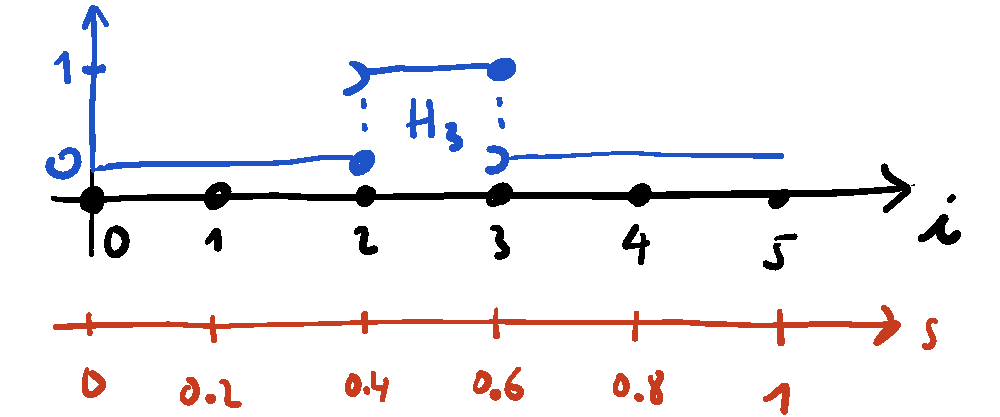
\includegraphics[width=0.95 \columnwidth]{base_functions}
\caption{\label{fig:base_functions}
---.}
\end{figure}
We introduce $N$ segments of equal size $h=1/N$, with $s_i=i \, h$ and $i \in (1;N)$, and use the following base functions, see Figure~\ref{fig:base_functions}
\begin{subequations}
 \label{eq:base_func}
\begin{align}
H_i(x) &= 1 \text{~ if ~} x_{i-1} \le x \le x_i  \\
H_i(x) &= 0 \text{~ otherwise ~}
\end{align}
\end{subequations}

The variation $\bar{\alpha}(x)$ and $\alpha(x)$ are represented as
\begin{subequations}
\label{eq:discrete_variations}
\begin{align}
\bar{\alpha}(s) &= \sum_{i=1}^N \bar{\alpha}_i \, H_i(s) \label{eq:19a} \\
\alpha(s) &= \sum_{i=1}^N \alpha_i \, H_i(s) \label{eq:19b}
\end{align}
\end{subequations}



We note $S=\int_0^1 s(\alpha) \d x$. The second variation in (\ref{eq:second_varia}) can then be written in matrix form as
\begin{subequations}
\begin{align}
\label{eq:second_varia_discrete}
\text{ for } i \neq j: \, H_{ij} = \Delta^2 \, h^2 \,  \frac{s'(\alpha_i) \, s'(\alpha_j)}{S^3} \\
%
H_{ii} = h\, W w''(\alpha_i) - \frac{\Delta^2}{2} \, h \,  \frac{s''(\alpha_i)}{S^2}  + \Delta^2 \, h^2 \,  \frac{s'(\alpha_i)^2}{S^3}
\end{align}
\end{subequations}
And the condition (\ref{eq:second_varia}) can be written as
\begin{align}
\label{eq:cond_second_varia_discrete}
\forall  \bar{\alpha}_i >0 \, , \forall  \bar{\alpha}_j >0  : \sum_{i,j} H_{ij} \, \alpha_i \, \alpha_j >0
\end{align}
this condition is fulfilled if
\begin{align}
\label{eq:cond_second_varia_discrete_bis}
\forall  i,j  :  H_{ij} >0
\end{align}




%
%
%
%
%
%
%
%
%
%% The Appendices part is started with the command \appendix;
%% appendix sections are then done as normal sections
%% \appendix

%% \section{}
%% \label{}

%% If you have bibdatabase file and want bibtex to generate the
%% bibitems, please use
%%

\bibliographystyle{elsarticle-harv}
\bibliography{discrete_damage}

\end{document}

\endinput
%%
%% End of file `elsarticle-template-harv.tex'.
